% docs/images/array_geometry.tex -- array of J antennas: geometric delay, beams, FOV, baseline (TikZ, standalone)
% Version 0.1.1 (2026-10-31): PNG rendering for notebook 00
%   (pdftoppm -r 160 -png -singlefile array_geometry.pdf array_geometry)
% Version 0.1.0 (2026-10-31): first version, redrawn in TikZ after a sketch
%   supplied by E. Schubert (a frequently reproduced figure of an antenna
%   array; original source to be named before publication).
% Build:  pdflatex array_geometry.tex   -> array_geometry.pdf
% Use in the documentation:  \includegraphics{images/array_geometry.pdf}
%   or (standalone package)  \includestandalone{images/array_geometry}
% ================================================================
\documentclass[tikz,border=2pt]{standalone}
\usepackage{amsmath}
\usetikzlibrary{arrows.meta,calc}

% ---------------------------------------------------------------- colours
\definecolor{skybg}{RGB}{230,230,255}
\definecolor{groundbg}{RGB}{214,247,214}
\definecolor{dishblue}{RGB}{107,166,209}
\definecolor{pedestal}{RGB}{10,10,110}
\definecolor{gainbox}{RGB}{255,255,0}

% ---------------------------------------------------------------- geometry
\def\dir{37}          % pointing direction (degrees above the horizon)
\def\dishy{0.75}      % height of the dish centre above the ground

\begin{document}
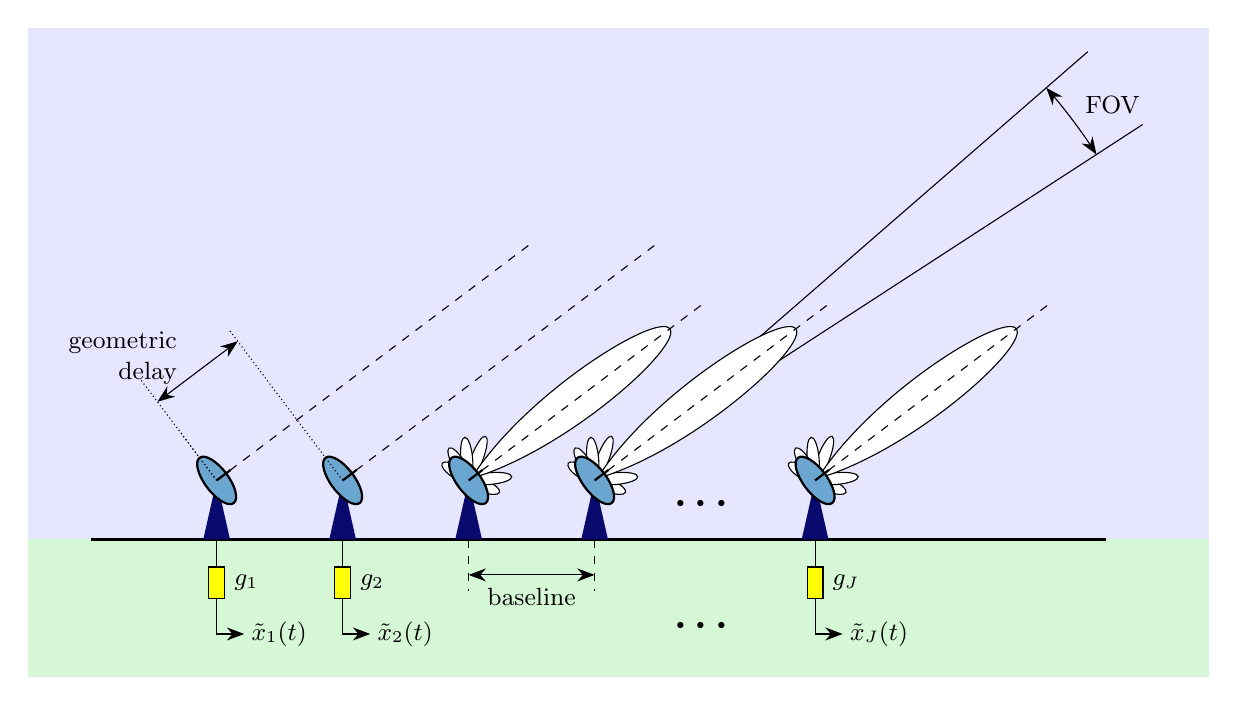
\begin{tikzpicture}[
    font=\small,
    >={Stealth[length=2.2mm]},
    wave/.style={densely dotted, thin},
    bore/.style={dashed, thin},
  ]

  % ------------------------------------------------------------ background
  \fill[skybg]    (-1.4,0) rectangle (13.6,6.5);
  \fill[groundbg] (-1.4,-1.75) rectangle (13.6,0);

  % ------------------------------------------------------------ antenna
  % \antenna{x}: pedestal (triangle) and dish (ellipse facing \dir)
  \newcommand{\antenna}[1]{%
    \fill[pedestal] (#1-0.17,0) -- (#1+0.17,0) -- (#1,0.75) -- cycle;
    \draw[thick, fill=dishblue, rotate around={\dir-90:(#1,\dishy)}]
      (#1,\dishy) ellipse (0.36 and 0.15);
    \draw[thick] (#1,\dishy) -- ++(\dir:0.22);
  }
  % \beam{x}: main lobe along \dir plus small side lobes
  \newcommand{\beam}[1]{%
    \foreach \a/\r in {-58/0.42, -32/0.55, 32/0.6, 58/0.55, 84/0.48, 110/0.4} {%
      \draw[fill=white, rotate around={\dir+\a:(#1,\dishy)}]
        (#1+0.5*\r,\dishy) ellipse ({0.5*\r} and 0.075);
    }
    \draw[fill=white, rotate around={\dir:(#1,\dishy)}]
      (#1+0.04,\dishy) .. controls +(1.2,0.45) and +(0,0.27) .. (#1+3.2,\dishy)
                       .. controls +(0,-0.27) and +(1.2,-0.45) .. (#1+0.04,\dishy);
    \draw[bore] (#1,\dishy) -- ++(\dir:3.75);
  }

  % ------------------------------------------------------------ ground line
  \draw[thick] (-0.6,0) -- (12.3,0);

  % ------------------------------------------------------------ antennas 1, 2 (without beams)
  \foreach \x in {1.0,2.6} {\draw[bore] (\x,\dishy) -- ++(\dir:5.0);}
  \antenna{1.0}
  \antenna{2.6}

  % wavefronts (perpendicular to the direction) through antennas 1 and 2
  \draw[wave] (1.0,\dishy) -- ++(\dir+90:0.75);
  \draw[wave] (2.6,\dishy) -- ++(\dir+90:2.40);
  % the geometric delay: distance between the two wavefronts along \dir
  \pgfmathsetmacro{\proj}{1.6*cos(\dir)}       % projection of the baseline
  \coordinate (d1) at ($(1.0,\dishy)+(\dir+90:1.25)$);
  \draw[<->] (d1) -- ++(\dir:\proj);
  \draw[wave] (1.0,\dishy) -- ++(\dir+90:1.6);
  \node[align=right, anchor=east] at ($(d1)+(\dir:0.5*\proj)+(\dir+90:0.15)+(-0.05,0.05)$)
    {geometric\\ delay};

  % ------------------------------------------------------------ antennas 3, 4, J (with beams)
  % field of view: two rays from antenna 4 with the FOV arc at their far end
  \draw (5.8,\dishy) -- ++(\dir+4:8.3) coordinate (f1);
  \draw (5.8,\dishy) -- ++(\dir-4:8.3) coordinate (f2);
  \draw[<->] ($(5.8,\dishy)+(\dir+4:7.6)$) arc[start angle=\dir+4, end angle=\dir-4, radius=7.6];
  \node[anchor=west] at ($(5.8,\dishy)+(\dir+1:7.75)$) {FOV};

  \foreach \x in {4.2,5.8,8.6} {\beam{\x} \antenna{\x}}

  % dots between antenna 4 and antenna J
  \node at (7.2,0.45) {\Large$\boldsymbol{\cdots}$};
  \node at (7.2,-1.1) {\Large$\boldsymbol{\cdots}$};

  % ------------------------------------------------------------ baseline between antennas 3 and 4
  \draw[dashed, thin] (4.2,0) -- (4.2,-0.65);
  \draw[dashed, thin] (5.8,0) -- (5.8,-0.65);
  \draw[<->] (4.2,-0.45) -- (5.8,-0.45);
  \node[anchor=north] at (5.0,-0.5) {baseline};

  % ------------------------------------------------------------ receiver chains g_k -> x_k(t)
  \foreach \x/\k in {1.0/1, 2.6/2, 8.6/J} {
    \draw (\x,0) -- (\x,-0.35);
    \draw[fill=gainbox] (\x-0.1,-0.35) rectangle (\x+0.1,-0.75);
    \node[anchor=west] at (\x+0.1,-0.55) {$g_{\k}$};
    \draw[->] (\x,-0.75) -- (\x,-1.2) -- (\x+0.35,-1.2);
    \node[anchor=west] at (\x+0.32,-1.2) {$\tilde{x}_{\k}(t)$};
  }
\end{tikzpicture}
\end{document}
